
% ------------------------------------------------------------------------
% ------------------------------------------------------------------------
% abnTeX2: Modelo de Trabalho Academico (tese de doutorado, dissertacao de
% mestrado e trabalhos monograficos em geral) em conformidade com 
% ABNT NBR 14724:2011: Informacao e documentacao - Trabalhos academicos -
% Apresentacao
% ------------------------------------------------------------------------
% ------------------------------------------------------------------------

\documentclass[
	% -- opções da classe memoir --
	12pt,				% tamanho da fonte
	openright,			% capítulos começam em pág ímpar (insere página vazia caso preciso)
	twoside,			% para impressão em recto e verso. Oposto a oneside
	a4paper,			% tamanho do papel. 
	% -- opções da classe abntex2 --
	%chapter=TITLE,		% títulos de capítulos convertidos em letras maiúsculas
	%section=TITLE,		% títulos de seções convertidos em letras maiúsculas
	%subsection=TITLE,	% títulos de subseções convertidos em letras maiúsculas
	%subsubsection=TITLE,% títulos de subsubseções convertidos em letras maiúsculas
	% -- opções do pacote babel --
	english,			% idioma adicional para hifenização
	french,				% idioma adicional para hifenização
	spanish,			% idioma adicional para hifenização
	brazil				% o último idioma é o principal do documento
	]{abntex2}

% ---
% Pacotes básicos 
% ---
\usepackage{lmodern}			% Usa a fonte Latin Modern			
\usepackage[T1]{fontenc}		% Selecao de codigos de fonte.
\usepackage[utf8]{inputenc}		% Codificacao do documento (conversão automática dos acentos)
\usepackage{lastpage}			% Usado pela Ficha catalográfica
\usepackage{indentfirst}		% Indenta o primeiro parágrafo de cada seção.
\usepackage{color}				% Controle das cores
\usepackage{graphicx}			% Inclusão de gráficos
\usepackage{microtype} 			% para melhorias de justificação
\usepackage{verbatim}
% ---

% code listing settings
\usepackage{listings}
\lstset{
    language=c,
    basicstyle=\ttfamily\scriptsize,
    aboveskip={1.0\baselineskip},
    belowskip={1.0\baselineskip},
    columns=fixed,
    extendedchars=true,
    breaklines=true,
    tabsize=4,
    prebreak=\raisebox{0ex}[0ex][0ex]{\ensuremath{\hookleftarrow}},
    frame=lines,
    showtabs=false,
    showspaces=false,
    showstringspaces=false,
    keywordstyle=\color[rgb]{0.627,0.126,0.941},
    commentstyle=\color[rgb]{0.133,0.545,0.133},
    stringstyle=\color[rgb]{01,0,0},
    numbers=left,
    numberstyle=\small,
    stepnumber=1,
    numbersep=15pt,
    captionpos=t,
    escapeinside={\%*}{*)}
}
		
% ---
% Pacotes adicionais, usados apenas no âmbito do Modelo Canônico do abnteX2
% ---
\usepackage{lipsum}				% para geração de dummy text
% ---

% ---
% Pacotes de citações
% ---
\usepackage[brazilian,hyperpageref]{backref}	 % Paginas com as citações na bibl
\usepackage[alf]{abntex2cite}	% Citações padrão ABNT

% --- 
% CONFIGURAÇÕES DE PACOTES
% --- 

% ---
% Configurações do pacote backref
% Usado sem a opção hyperpageref de backref
\renewcommand{\backrefpagesname}{Citado na(s) página(s):~}
% Texto padrão antes do número das páginas
\renewcommand{\backref}{}
% Define os textos da citação
\renewcommand*{\backrefalt}[4]{
	\ifcase #1 %
		Nenhuma citação no texto.%
	\or
		Citado na página #2.%
	\else
		Citado #1 vezes nas páginas #2.%
	\fi}%
% ---

% ---
% Informações de dados para CAPA e FOLHA DE ROSTO
% ---
\titulo{Projeto Final de Microprocessadores II}
\autor{Evandro Viva \and Isaías Lima \and Patrícia Fabbri}
\local{Brasil}
\data{2017, v-1.0.0}
\orientador{Prof. Ivair Neves Abreu}
\instituicao{%
  Universidade Presbiteriana Mackenzie - UPM
  \par
  Escola de Engenharia
  \par
  Microprocessadores II}
\tipotrabalho{Projeto Final}
% O preambulo deve conter o tipo do trabalho, o objetivo, 
% o nome da instituição e a área de concentração 
\preambulo{Apresentação de proposta de valor, público alvo, conhecimentos técnicos e aprendizado desenvolvido aplicados na construção de uma solução corporativa.}
% ---


% ---
% Configurações de aparência do PDF final

% alterando o aspecto da cor azul
\definecolor{blue}{RGB}{41,5,195}

% informações do PDF
\makeatletter
\hypersetup{
     	%pagebackref=true,
		pdftitle={\@title}, 
		pdfauthor={\@author},
    	pdfsubject={\imprimirpreambulo},
	    pdfcreator={LaTeX with abnTeX2},
		pdfkeywords={iot}{ibeacon}{arduino}{microprocessadores}{empreendedorismo}, 
		colorlinks=true,       		% false: boxed links; true: colored links
    	linkcolor=blue,          	% color of internal links
    	citecolor=blue,        		% color of links to bibliography
    	filecolor=magenta,      		% color of file links
		urlcolor=blue,
		bookmarksdepth=4
}
\makeatother
% --- 

% --- 
% Espaçamentos entre linhas e parágrafos 
% --- 

% O tamanho do parágrafo é dado por:
\setlength{\parindent}{1.5cm}

% Controle do espaçamento entre um parágrafo e outro:
\setlength{\parskip}{0.0cm}  % tente também \onelineskip

% ---
% compila o indice
% ---
\makeindex
% ---

% ----
% Início do documento
% ----
\begin{document}

% Seleciona o idioma do documento (conforme pacotes do babel)
%\selectlanguage{english}
\selectlanguage{brazil}

% Retira espaço extra obsoleto entre as frases.
\frenchspacing 

% ----------------------------------------------------------
% ELEMENTOS PRÉ-TEXTUAIS
% ----------------------------------------------------------
% \pretextual

% ---
% Capa
% ---
\imprimircapa
% ---

% ---
% Folha de rosto
% (o * indica que haverá a ficha bibliográfica)
% ---
\imprimirfolhaderosto*
% ---

% ---
% Inserir a ficha bibliografica
% ---

% Isto é um exemplo de Ficha Catalográfica, ou ``Dados internacionais de
% catalogação-na-publicação''. Você pode utilizar este modelo como referência. 
% Porém, provavelmente a biblioteca da sua universidade lhe fornecerá um PDF
% com a ficha catalográfica definitiva após a defesa do trabalho. Quando estiver
% com o documento, salve-o como PDF no diretório do seu projeto e substitua todo
% o conteúdo de implementação deste arquivo pelo comando abaixo:
%
% \begin{fichacatalografica}
%     \includepdf{fig_ficha_catalografica.pdf}
% \end{fichacatalografica}

\begin{fichacatalografica}
	\sffamily
	\vspace*{\fill}					% Posição vertical
	\begin{center}					% Minipage Centralizado
	\fbox{\begin{minipage}[c][8cm]{13.5cm}		% Largura
	\small
	\imprimirautor
	%Sobrenome, Nome do autor
	
	\hspace{0.5cm} \imprimirtitulo  / \imprimirautor. --
	\imprimirlocal, \imprimirdata-
	
	\hspace{0.5cm} \pageref{LastPage} p. : il. (algumas color.) ; 30 cm.\\
	
	\hspace{0.5cm} \imprimirorientadorRotulo~\imprimirorientador\\
	
	\hspace{0.5cm}
	\parbox[t]{\textwidth}{\imprimirtipotrabalho~--~\imprimirinstituicao,
	\imprimirdata.}\\
	
	\hspace{0.5cm}
		1. Internet of Things.
		2. Arduino.
		2. iBeacon.
		I. Prof. Ivair Neves Abreu.
		II. Universidade Presbiteriana Mackenzie.
		III. Escola de Engenharia.
		IV. Projeto Final de Microprocessadores II 			
	\end{minipage}}
	\end{center}
\end{fichacatalografica}
\newpage
% ---

% ---
% Inserir folha de aprovação
% ---

% ---
% Dedicatória
% ---
\begin{dedicatoria}
   \vspace*{\fill}
   \centering
   \noindent
   \textit{ Este trabalho é dedicado aos jovens engenheiros que decidiram transformar o mundo onde vivem através da tecnologia.} \vspace*{\fill}
\end{dedicatoria}
% ---

% ---
% RESUMOS
% ---

% resumo em português
\setlength{\absparsep}{18pt} % ajusta o espaçamento dos parágrafos do resumo
\begin{resumo}
Visando desenvolver soluções que apliquem os conhecimentos da matéria, é possível aplicar a tecnologia \emph{iBeacon}, variante do sistema \emph{Bluetooth}, para auxiliar empresas que desejem manter o controle da localização dos computadores móveis associados aos funcionários, utilizando os benefícios do \emph{Arduino}, da Internet das Coisas e dos conceitos de empreendedorismo. Sabendo do que estas empresas precisam, é possível estruturar o sistema microprocessado, listar o \emph{hardware} necessário para o seu desenvolvimento, montar o protótipo e obter o início do que pode ser uma solução simples e de grande valia para o meio corporativo.

 \textbf{Palavras-chave}: IoT. iBeacon. Arduino.
\end{resumo}

% ---
% inserir lista de ilustrações
% ---
\pdfbookmark[0]{\listfigurename}{lof}
\listoffigures*
\newpage
% ---

% ---
% inserir lista de tabelas
% ---
\pdfbookmark[0]{\listtablename}{lot}
\listoftables*
\newpage
% ---

% ---
% inserir lista de abreviaturas e siglas
% ---
\begin{siglas}
  \item[IoT] \emph{Internet of Things}
  \item[EEPROM] \emph{Electrically Erasable Programmable Read-Only Memory}
  \item[BLE] \emph{Bluetooth Low Energy}
  \item[MQQT] \emph{Message Queue Telemetry Transport}
  \item[AWS] \emph{Amazon Web Services}
  \item[CBL] \emph{Challenge Based Learning}
  \item[SSID] \emph{Service Set Identifier}
  \item[WWDC] \emph{World Wide Developer Conference}
  \item[UUID] \emph{Universally Unique Identifier}
  \item[IDE] \emph{Integrated Development Environment}
  \item[IEEE] \emph{Institute of Electrical and Electronics Engineers}
\end{siglas}
% ---

% ---
% inserir o sumario
% ---
\pdfbookmark[0]{\contentsname}{toc}
\tableofcontents*
\newpage
% ---



% ----------------------------------------------------------
% ELEMENTOS TEXTUAIS
% ----------------------------------------------------------
\textual

% ----------------------------------------------------------
% Introdução (exemplo de capítulo sem numeração, mas presente no Sumário)
% ----------------------------------------------------------
\chapter*[Introdução]{Introdução}
\addcontentsline{toc}{chapter}{Introdução}
% ----------------------------------------------------------

Diante da facilidade oferecida pelo mercado de tecnologia, é fato que qualquer um pode programar, montar um \emph{hardware} e desenvolver soluções, mas também é verdade que, para obtenção de melhores resultados, a construção de conhecimentos em programação, microprocessadores e IoT mais voltados para a Engenharia é uma base indispensável. É através dessas bases que o presente trabalho visa demonstrar, passo a passo, como uma solução \emph{Businees to Business} pode ser desenvolvida, explicando o passo a passo da concepção do problema, a sugestão de uma solução e todo o pensamento técnico por trás dela.

Através de princípios do empreededorismo, a dor de uma empresa é fonte de uma oportunidade. Como é o cotiano dela? O que ela precisa realizar, quais as suas metas? Quais as dores que ela enfrenta neste processo?

Através dos conhecimentos da Engenharia, a solução surge, unindo as bases teóricas num sistema com novas aplicações. Como as tecnologias conhecidas poderiam atuar neste problema? O que pode ser combinado? Qual o trabalho envolvido em unir estes dispositivos?

Através da Computação, a solução é revestida de recursos que a integram ao universo presente de modo que comece a resolver o problema. Um servidor é necessário para receber os dados? É necessária a autenticação? O sistema precisa de criptografia forte? Suas informações são confidenciais? Deveria ser acessíveis de qualquer local?

% ----------------------------------------------------------
% PARTE
% ----------------------------------------------------------
\part{Prospecção do Problema}
% ----------------------------------------------------------

\chapter{CBL}

Toda pesquisa começa com observação e, limitando o escopo por causa dos prazos, a observação inicial foi concentrada na empresa P\&G, produtora de bens de consumo em geral, mais especificamente em seu departamento de Tecnologia da Informação, onde um dos pesquisadores é estagiário. Através destas observações, é possível desenvolver o pensamento CBL, levantando vários questionamentos em função de um tema, uma questão central e um desafio (respectivamente: área do conhecimento, a pergunta central a ser respondida e a meta que levará a essa resposta).

\textbf{Tema Central:} Internet das Coisas.

\textbf{Questão Essencial:} Como auxiliar empresas a terem controle dos seus computadores?

\textbf{Desafio:} Produzir um sistema que auxilie empresas a terem o controle sobre seus computadores e demais dispositivos.

\section{Questões Norteadoras}

Diante do CBL que envolve o projeto, é possível realizar perguntas que direcionam o desenvolvimento da solução, que são respondidas através da observação, do questionamento e da reflexão pessoal:

\begin{enumerate}
    \item Quais são as tarefas que um funcionário realiza? 
    \item Quais são as tarefas que a empresa precisa realizar?
    \item O ativo de um computador é associado a um funcionário?
    \item Se o empregado atinge seus objetivos, o que ele ganha?
    \item Se a empresa cumpre suas metas, o que ela ganha?
    \item Quais as dores envolvidas tanto para funcionários quando para empresas no processo?
    \item O que acontece no caso de um funcionário perder ou danificar a máquina?
    \item Como a empresa protege seu patrimônio nessas situações?
    \item Essa restituição contratual dá certo?
\end{enumerate}

Feitas as perguntas, e seguindo o que foi levantado, eis suas respostas:

\begin{enumerate}
    \item Simulações, planilhas, assistêcia técnica, conferências, relatórios, cálculos, atendimento, recursos humanos, etc
    \item Vendas, metas dos investidores, produtividade, melhora do produto, controle de qualidade, etc.
    \item Em muitas empresas, sim, pois o funcionário muitas vezes precisa levar consigo o computador para finalizar tarefas em sua própria residência.
    \item Salário, benefícios, estabilidade, promoções, estima da liderança, perspectivas.
    \item Aumento das vendas, mais investimentos, crescimento, novos clientes, aumento do valor de mercado.
    \item Se o funcionário falha, pode perder seu emprego e dar prejuízo para a empresa, que pára de focar no essencial para resolver problemas menores e gastar dinheiro neles se for o caso.
    \item A empresa cobra do funcionário o valor referente ao equipamento e restitui seu ativo.
    \item Através de um contrato formal entre empresa e funcionário, associando a cada uma das partes seus direitos e deveres.
    \item Caso a empresa tenha um grande arquivo e acabe não encontrando o contrato firmado, pode ter de arcar com as despesas do equipamento e até pode gastar mais se for demitir um empregado.
\end{enumerate}

\section{Análise}

Diante das questões levantadas, é possível perceber que há uma brecha neste processo. Caso um funcionário perca o ativo e o contrato não seja encontrado, a companhia tem um prejuízo para restituir seu patrimônio, perdendo dinheiro e tempo fora do que ela considera essencial para seu funcionamento. Ou seja, ela precisa manter um controle correto e sólido de seus ativos e de seus contratos para saber quem está designado ao equipamento e garantir que esta pessoa seja responsabilizada por ele (além de garantir que a pessoa certa seja responsabilizada).

Sendo assim, uma dor surge, que precisa de uma solução que: resolva, obviamente, o problema; seja viável e de fácil implementação; e que exija o mínimo de treinamento novo de seu pessoal, já que isso, fato observado no cotidiano pelos pesquisadores, gera um período de adaptação que pode ser incômodo e caro.

\chapter{Solução}

Os conhecimentos técnicos dos pesquisadores permitem que o problema seja solucionado através de tecnologias. Para tanto, é necessário que novas questões norteadoras sejam realizadas (vale ressaltar que algumas perguntas surgem das respostas das anteriores).

\section{Questões Norteadoras}

\begin{enumerate}
    \item O controle de dispositivos envolve que práticas?
    \item É possível localizar um computador através do GPS? E se ele estiver desligado?
    \item Com o computador desligado, como continuar obtendo sua localização?
    \item Quais são as alternativas do mercado ao GPS?
    \item Estas alternativas permitem maior precisão na localização?
    \item É realmente necessário saber a localização precisa do dsipositivo?
\end{enumerate}

Feitas as perguntas, novamente suas respostas:

\begin{enumerate}
    \item Localização, registro, monitoramento, etc.
    \item Com o computador desligado, o Wi-Fi já permite saber onde ele está. Se ele estiver fora da tomada e desligado, não há como obter sua ocalização.
    \item Emissor externo de localização.
    \item \emph{iBeacon}, se o caso for encontrar algo barato e de fácil implementação.
    \item Sim.
    \item De acordo com as empresas, só sabendo se ele está ou não no espaço físico já é necessário.
\end{enumerate}

\section{Análise}

Analisando estas respostas, então é possível ver que algum tipo de \emph{tag} colada no computador, como um \emph{iBeacon}, poderia ser a solução para os problemas observados. Mas quais os equipamentos e qual o \emph{hardware} necessários para que um sistema baseado nesta ideia se desenvolva. Com a solução em mãos e com os conhecimentos técnicos de Microprocessadores, os pesquisadores puderam realizar seu projeto final.

\part{Desenvolvimento da Solução}

\chapter{Resumindo o sistema}

Sabendo do que as empresas precisam, a proposta do sistema é o resumo do que precisa ser desenvolvido.

\section{Sistema}

Já que é necessário saber se o computador está na empresa, um \emph{iBeacon} colocado na máquina pode enviar sua localização para três \textbf{centrais}, que triangulam sua posição e sabem se ele está deixando ou chegando na empresa. Estas centrais estariam conversando com um \textbf{servidor}, comunicando-o sobre o horário e o identificador do computador que saiu ou entrou na empresa. O servidor, por sua vez, tendo esse identificador catalogado em seu banco de dados, seria capaz de associar o registro a um funcionário, assim permitindo à empresa ter provas de quem é o dono do ativo e tomar providências em qualquer caso.

\section{Requisitos}

Para um \emph{iBeacon} a prática é simples, dado que ele é um dispositivo unificado de fácil acesso e de entendimento simples, que será detalhado mais adiante. 

A central precisa de: uma EEPROM, para armazenar suas chaves de acesso ao Wi-Fi; um transceptor BLE HM10, para comunicação com a \emph{tag}; um microcontrolador ESP8266 (que embarca módulo de conexão Wi-Fi), semelhante ao Arduino, para implementação a lógica; e uma fonte de energia constante qualquer.

O servidor precisa de: uma programação, implementada através do Node JS; um protocolo de comunicação, feito por MQTT; uma hospedagem, feita pelo AWS e simulada num \textit{Raspberry Pi} junto a um roteador para a apresentação.

\section{Funcionamento}

Primeiro, o ESP8266 tenta se concetar ao Wi-Fi através do SSID armazenado na EEPROM e, caso não consiga, abre um servidor para que um usuário possa realizar um \emph{post} com os dados de acesso da rede. Se estiver conectado, tenta se conectar ao servidor via MQTT e, tendo obtido sucesso, tenta se conectar ao HM10 para procurar dispositivos ao redor. Tendo achado os dispositivos, envia os dados de distância obtidos por triangulação após perguntar ao servidor se reconhece cada um deles.

\begin{figure}[t]
    \centering
    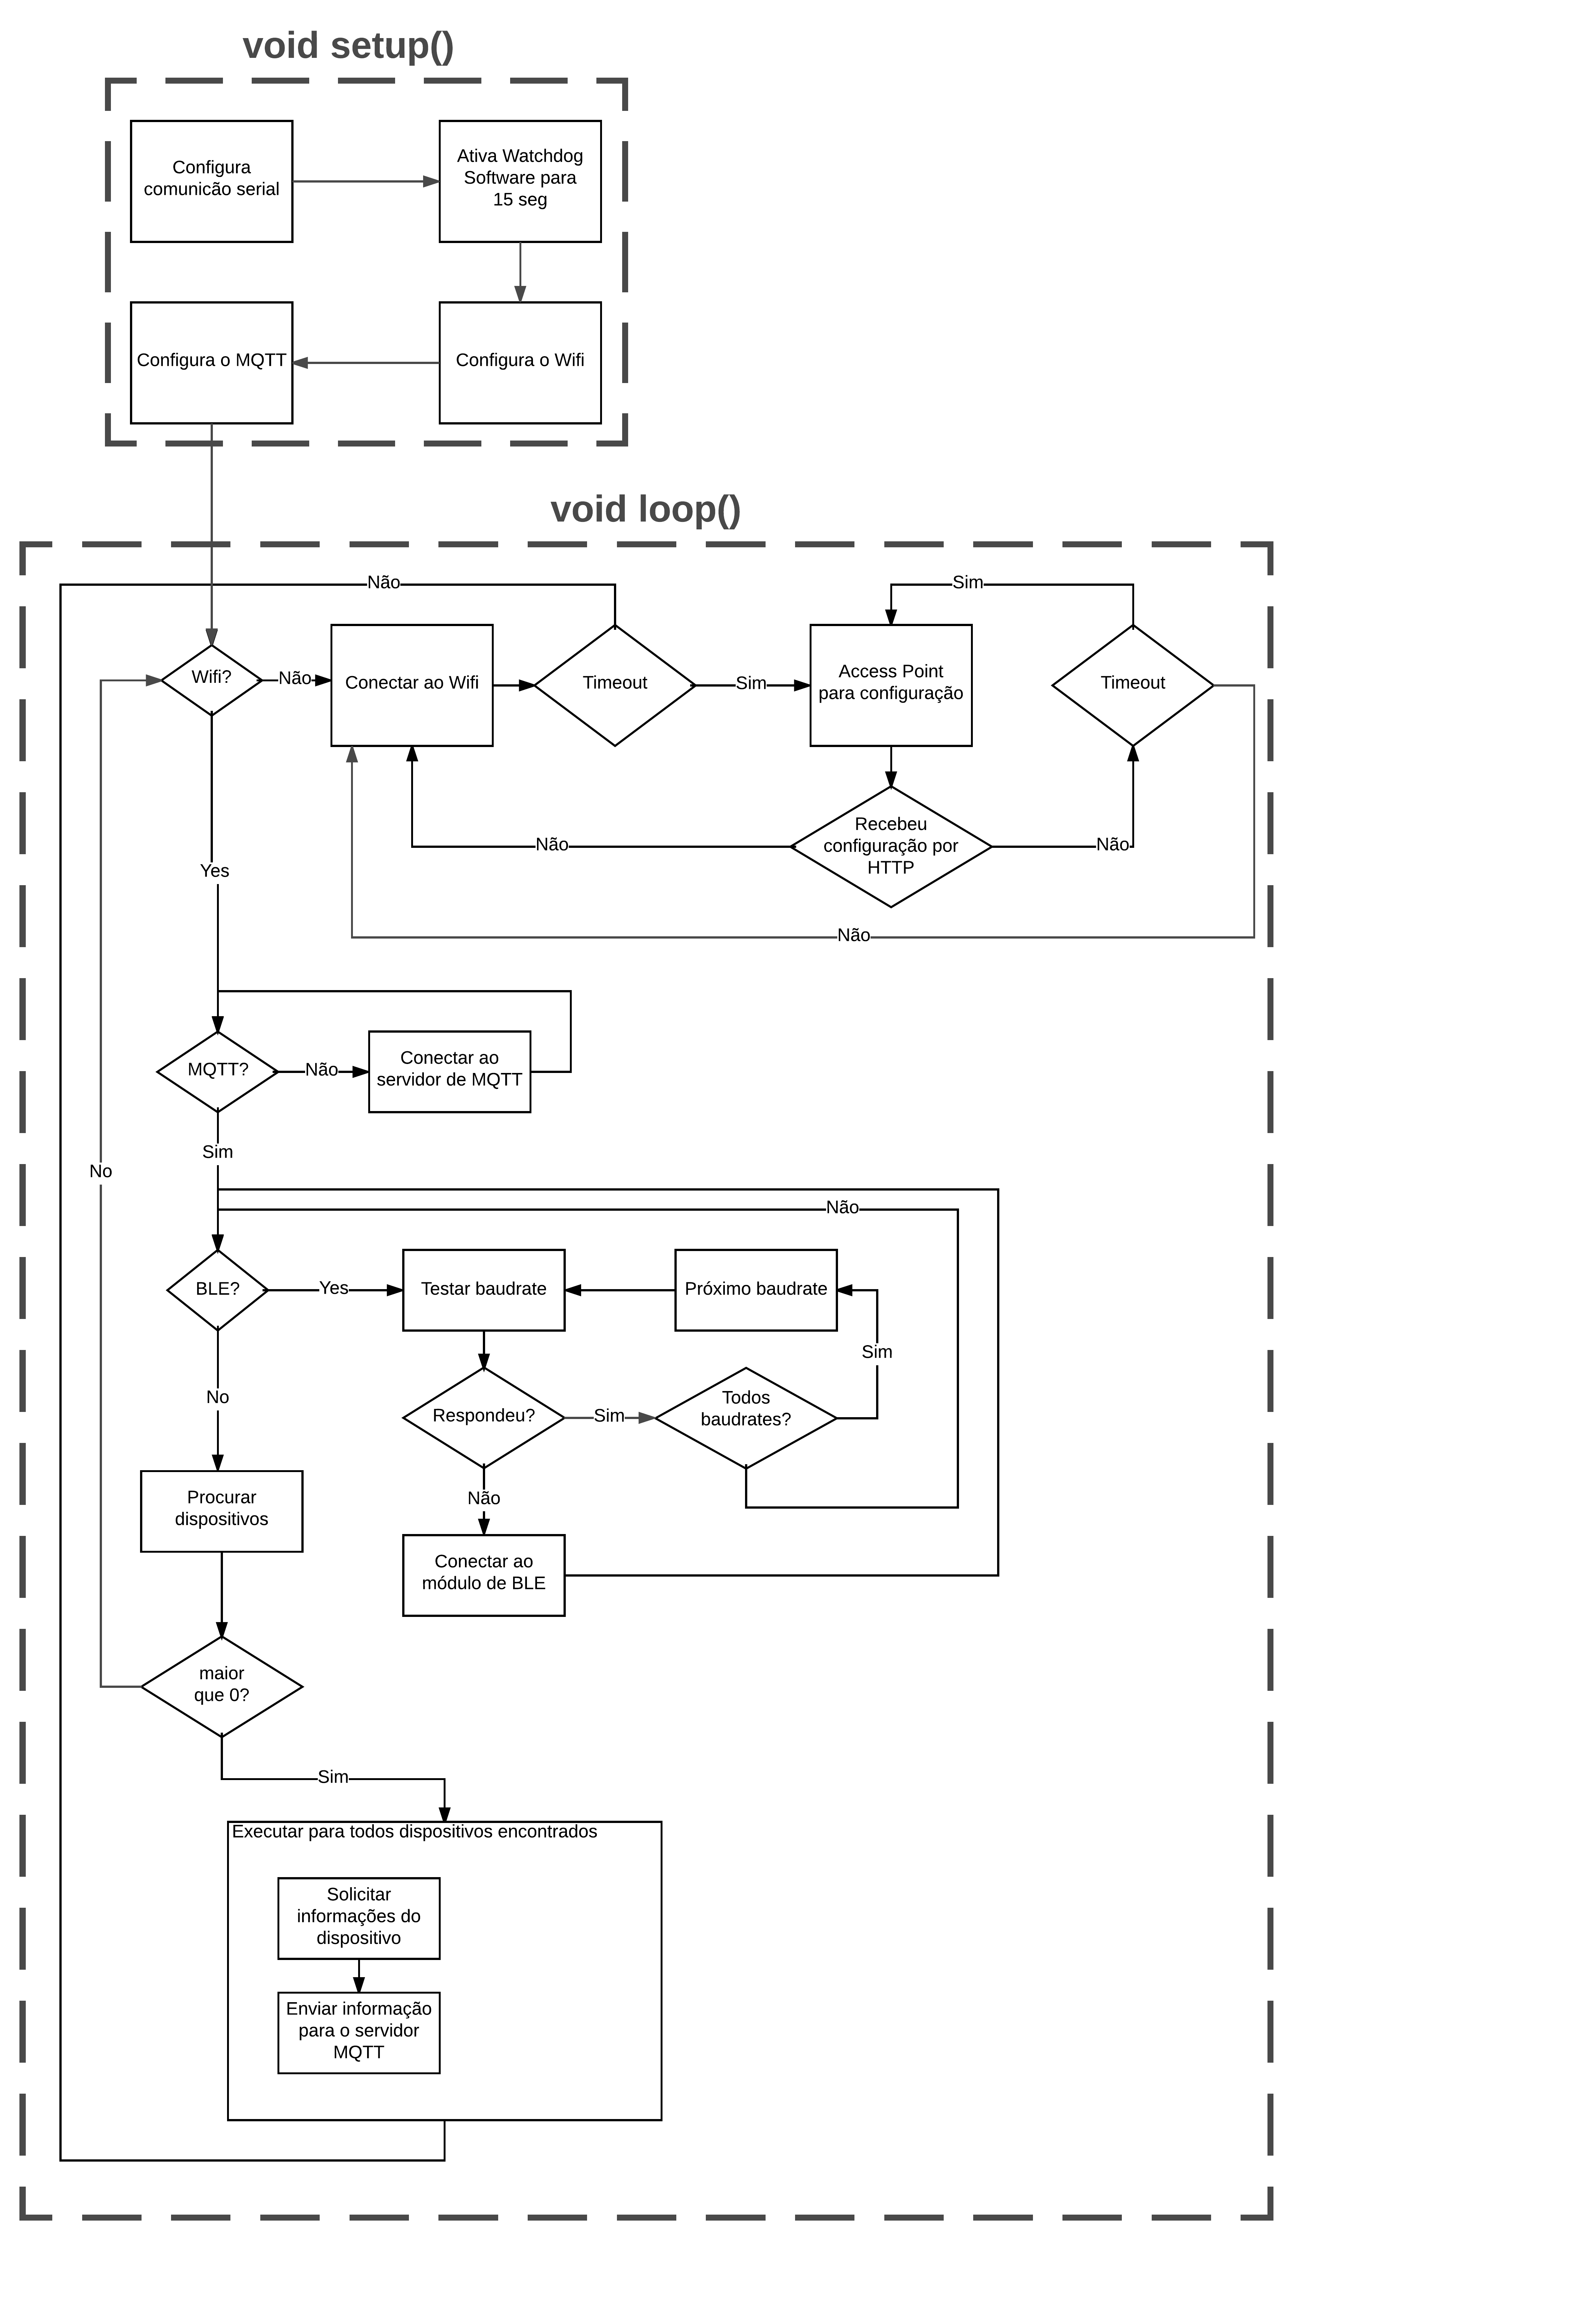
\includegraphics[width=\linewidth]{block_diagram}
    \caption{Algoritmo lógico do sistema.}
    \label{fig:blocos}
\end{figure}

\chapter{Detalhes Técnicos}

\section{\emph{iBeacon}}

Lançado na WWDC de 2013, implementa as funcionalidades do BLE emitindo três sinais: um UUID de 16 bytes, um \emph{major} e um \emph{minor} de 2 bytes cada e mais outros sinais indicando o nível do sinal, o fabricante, etc, como pode ser visto no \emph{snippet} a seguir:

\begin{verbatim}
    Byte 0: Length :  0x02
    Byte 1: Type: 0x01 (Flags)
    Byte 2: Value: 0x06 (Typical Flags)
    Byte 3: Length: 0x1a
    Byte 4: Type: 0xff (Custom Manufacturer Packet)
    Byte 5-6: Manufacturer ID : 0x4c00 (Apple)
    Byte 7: SubType: 0x2 (iBeacon)
    Byte 8: SubType Length: 0x15
    Byte 9-24: Proximity UUID
    Byte 25-26: Major
    Byte 27-28: Minor
    Byte 29: Signal Power
\end{verbatim}

\begin{table}[h!]
    \centering
    \begin{tabular}{ | l | l | } 
        \hline
        MCU                             & Bluetooth SoC \\
                                        & ARM Cortex-M4 32-bit processor with FPU \\
                                        & 64 MHz Core Speed \\
                                        & 512 kB Flash Memory \\
                                        & 64 kB RAM Memory \\
        \hline
        Radio2.4 GHz transceiver        & Bluetooth 4.2 LE Standard \\
                                        & Range: up to 200 meters \\
                                        & Output power: -20 to +4 dBm in 4 dB steps, \\
                                        & ``Whisper mode'' -40 dBm, \\
                                        & ``Long range mode'' +10 dBm \\
                                        & Sensitivity: -96 dBm \\
                                        & Frequency range: 2400 MHz to 2483.5 Mhz \\
                                        & 40 channels \\
                                        & Adjacente channel separation: 2 MHz \\
                                        & Modulation: GFSK (FHSS) \\
                                        & Antenna: PCB Meander, Monopole \\
                                        & Antenna gain: 0 dBi \\
                                        & Over-the-air data rate: 1 Mbps (2 Mbps supported) \\
        \hline
        Sensors                         & Motion sensor (3-axis) \\
                                        & Temperature sensor \\
                                        & Ambient Light sensor \\
                                        & Magnetometer (3-axis) \\
                                        & Pressure sensor \\
                                        & EEPROM Memory 1 Mb \\
                                        & RTC clock \\
        \hline
        Additional Features             & GPIO \\
                                        & NFC \\
        \hline
        Power Supply                    & 4 x CR2477 – 3.0V lithium primary cell battery (replaceable) \\
                                        & High efficient Step-Down DC-DC converter \\
        \hline
        Environmental Specification     & Operating Temperature: 0 to 60 degrees Celsius \\
                                        & Storage Temperature (recommended): 15 to 30 degrees Celsius \\
                                        & Relative Humidity (operating): 20\% to 80\% relative humidity \\
                                        & Relative Humidity (storage): 10\% to 90\% relative humidity, \\
                                        & non-condensing \\
                                        & Splash-proof \\
        \hline
        Materials                       & non-flammable \\
                                        & enclosure: silicone \\
                                        & adhesive layer: double-sided adhesive tape \\
        \hline
        Measures                        & Length: 62.7 mm (2.47 inches) \\
                                        & Width: 41.2 mm (1.62 inches) \\
                                        & Height: 23.6 mm (0.93 inches) \\
                                        & Weight: 67g (2.36 ounces) \\
        \hline
    \end{tabular}
    \caption{Especificações Técnicas \textit{iBeacon} Estimote}
    \label{table:ibeacon}
\end{table}

Os bytes de 0 a 2 são os normalmente emitidos pelo BLE, sendo que os demais são os acrescentados pelo \emph{iBeacon}. 

O dispositivo pode ser vendido em vários formatos e cores, atualmente tornando-se popular entre os desenvolvedores e encontrando aplicações além do varejo (emissão de anúncios). Um dos maiores fabricantes é a Estimote, oferecendo \emph{kits} de desenvolvimento iOS com algumas \emph{tags}, mas qualquer \textit{iPhone} pode emitir um sinal com o protocolo (alguns aplicativos da loja da Apple já são voltados para este propósito).

\section{HM10}

o BLE HM10 é um módulo que pode ser conectado ao WEMOS, sendo um transceptor de sinal \textit{Bluetooth} do mesmo modo que o \textit{iBeacon}. Possui seis \textit{ports} acessíveis, como mostrado na Tabela \ref{table:hm10}, comunicando-se serialmente com o microcontrolador e recebendo alimentação deste também. A Figura \ref{fig:hm10} ilustra com maiores detalhes seus demais \textit{ports}. 

\begin{table}[t!]
    \centering
    \begin{tabular}{ | c  r | } 
        \hline
                        & STATE \\
                        & VCC \\
                        & GND \\
                        & TX \\
                        & RX \\
                        & BRK \\
        \hline
    \end{tabular}
    \caption{\textit{Ports} do módulo HM10}
    \label{table:hm10}
\end{table}

\begin{figure}[h]
    \centering
    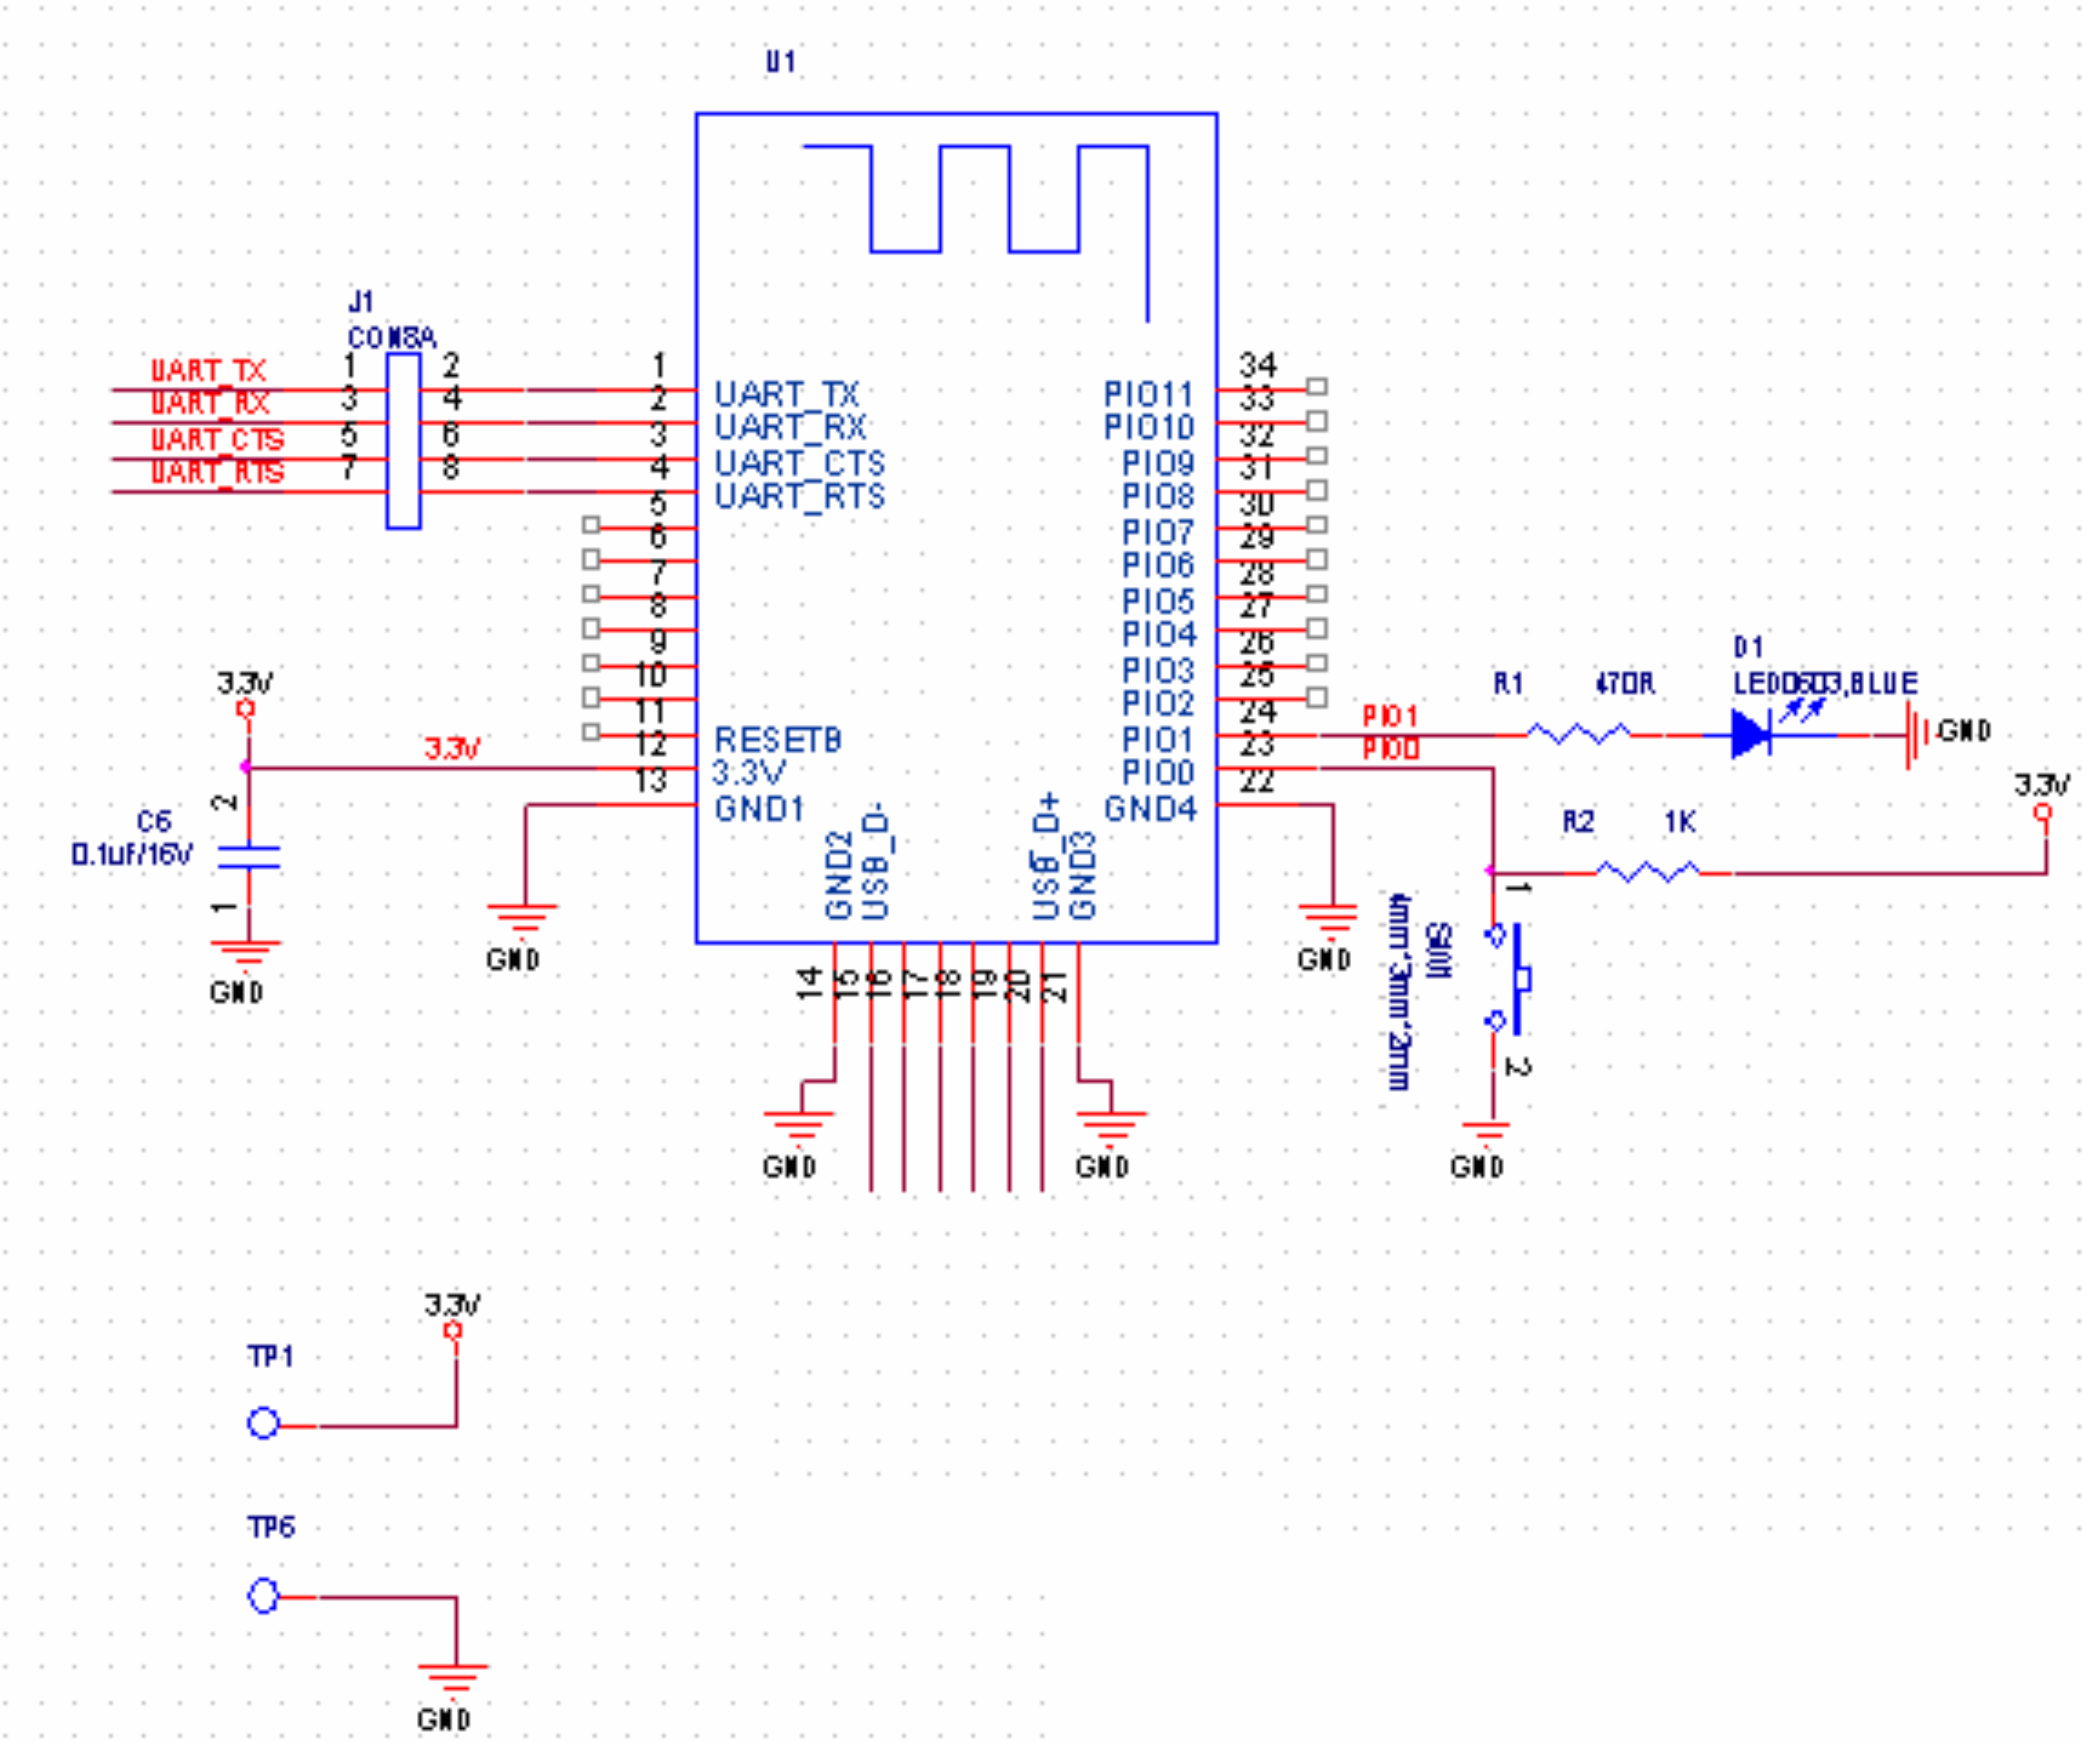
\includegraphics[width=\linewidth]{hm-10-pinout}
    \caption{Diagrama lógico do módulo HM10.}
    \label{fig:hm10}
\end{figure}

\section{ESP8266 e WEMOS}

O ESP8266 é um módulo de conexão Wi-Fi que embute em suas funcionalidades um microcontrolador que pode ser programado pelo IDE do Arduino, graças ao WEMOS, conjunto que embarca o módulo e inclui um conversor USB Serial, regulador de tensão e botão de \textit{reset}. o ESP8266 possui uma EEPROM emulada por \textit{software} e uma memória \textit{Flash}, além de \textit{watch dog} implementado via \textit{software} e \textit{hardware} que dispara após 15 segundos (não pode ser alterado), vide \citeonline{esp8266}.

\begin{figure}[t!]
    \centering
    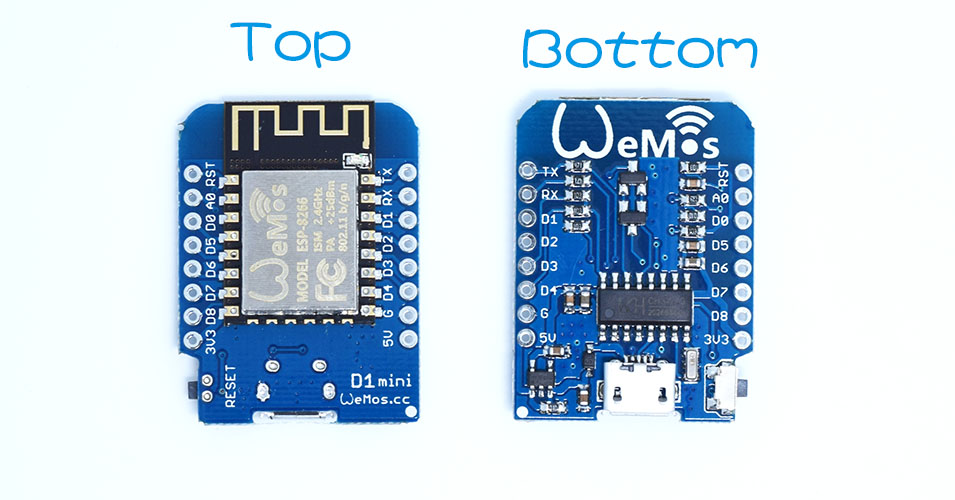
\includegraphics[width=\linewidth]{wemos-pinout}
    \caption{\textit{Ports} e esquema do \textit{chip} WEMOS, com ESP8266 embutido.}
    \label{fig:hm10}
\end{figure}

\begin{figure}[h!]
    \centering
    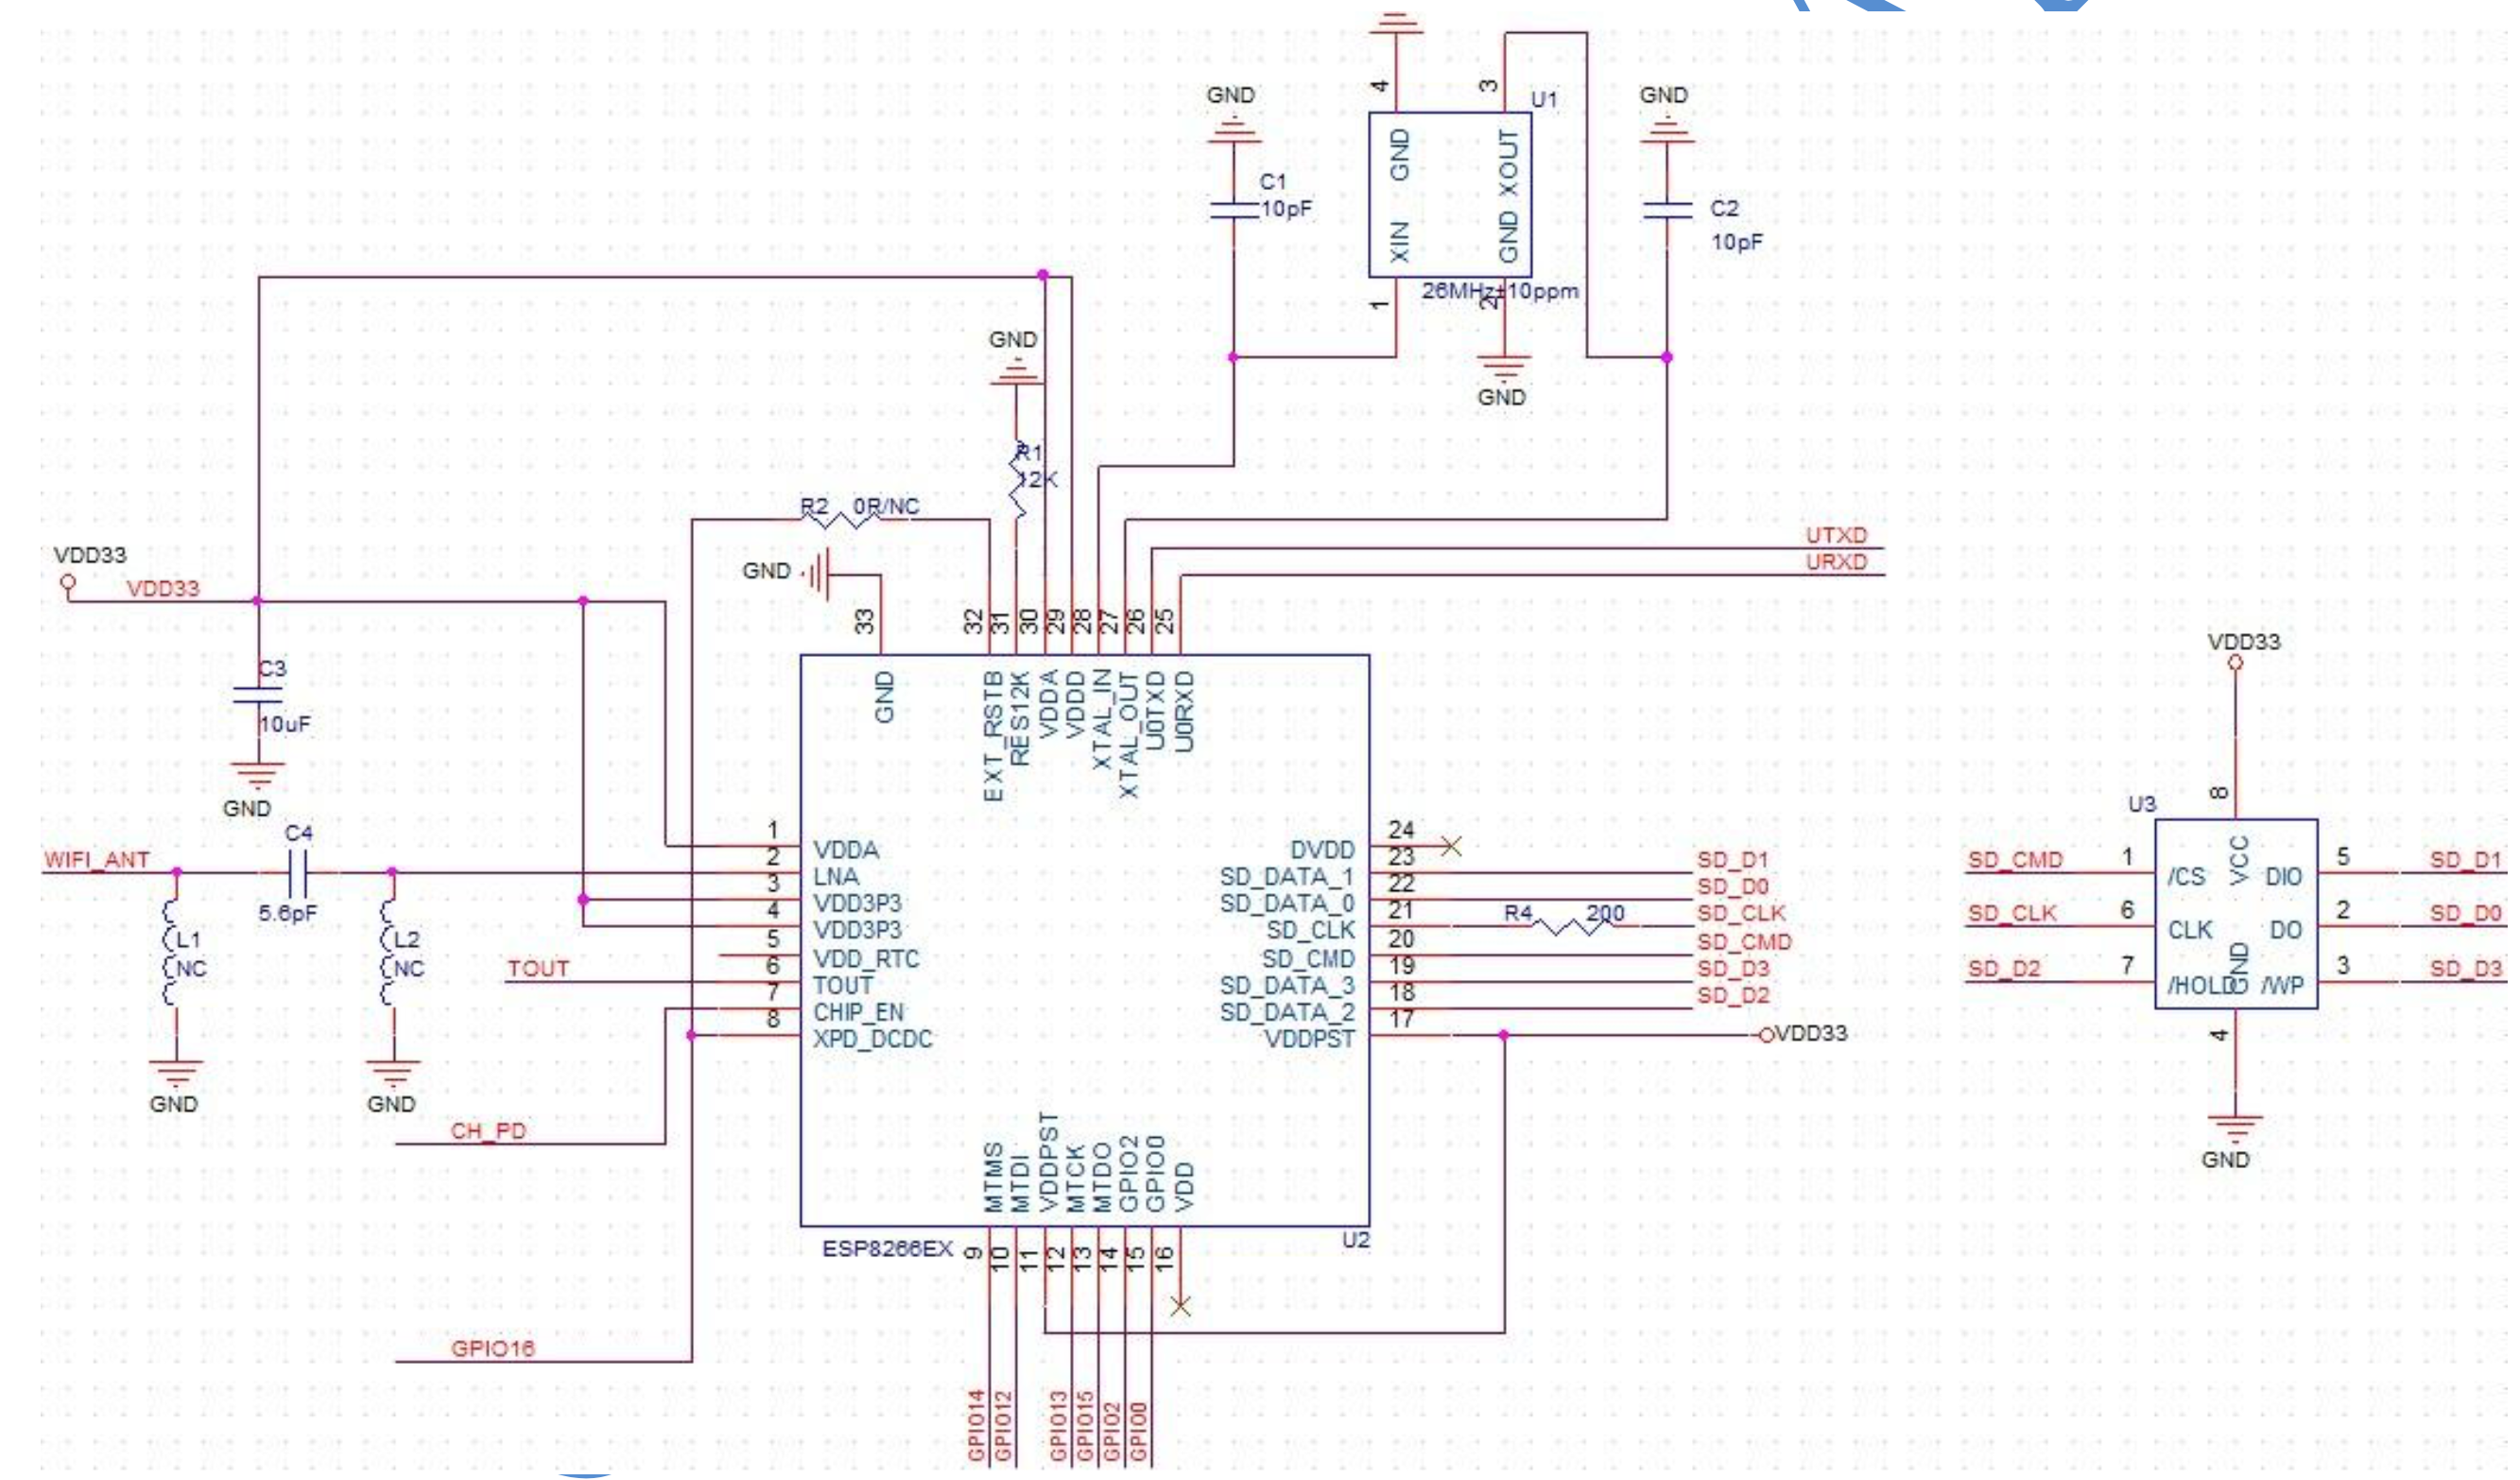
\includegraphics[width=\linewidth]{esp8266}
    \caption{Esquema do ESP8266.}
    \label{fig:esp8266}
\end{figure}

\section{MQTT}

O MQTT é um protocolo para mensagens ``leve'' para pequenos dispositivos móveis otimizado para redes TCP/IP não confiáveis ou de média latência, com modelo de troca de informações baseado no modelo publicador-subscriptor, que substitui o HTTP em aplicações desse porte, vide \citeonline{wiki:mqtt}. A Tabela \ref{table:mqtt} mostra os métodos do protocolo.

\begin{table}[h]
    \centering
    \begin{tabular}{ | r  l | } 
        \hline
            CONNECT & Cliente solicita uma ligação com um servidor \\
            CONNACK & Reconhece solicitação de conexão \\
            PUBLISH & publicar mensagem \\
            PUBACK & reconhecimento de publicação \\
            PUBREC & Publicação recebida.(QoS 2 Publicação recebida., part 1) \\
            PUBREL & Publicação publicada. (QoS 2 Publicação recebida., part 2) \\
            PUBCOMP & Publicação completada. (QoS 2 Publicação recebida., part 3) \\
            SUBSCRIBE & Inscrever-se em um tópico \\
            SUBACK & Reconhecimento de inscrição \\ 
            UNSUBSCRIBE & Cancelamento de inscrição em um tópico \\
            UNSUBACK & Reconhecimento de cancelamento de inscrição. \\
            PINGREQ & PING request \\
            PINGRESP & PING response \\
            DISCONNECT & Notificação de desconecção \\
        \hline
    \end{tabular}
    \caption{Métodos MQTT}
    \label{table:mqtt}
\end{table}

\section{Node JS}

É um intepretador do \textit{Java Script} que funciona do lado do servidor, auxiliando programadores a implementar servidores e alta escalabilidade que suportem dezenas de milhares de conexões simultâneas numa única máquina. Ele é baseado no interpretador implementado em C++ pela Google, usado no \textit{Chrome}, tendo sido criado em 2009, vide \citeonline{nodejs}.

\chapter{O sistema completo}

Possuindo conhecimento de todas as partes envolvidas no sistema, baseando-se no resumo e aplicando os conhecimentos de Microprocessadores, é possível detalhar de modo completo a união dos componentes e seus resultados.

\section{Central}

A central é responsável por monitorar e observar os \textit{iBeacons}. Detalhando melhor o que foi dito no resumo, é constituída por um WEMOS (ESP8266 embarcado) conectado serialmente ao módulo HM10 e alimentado por fonte USB comum. A Figura \ref{fig:central} ilustra a ligação dos componentes.

\begin{figure}[h!]
    \centering
    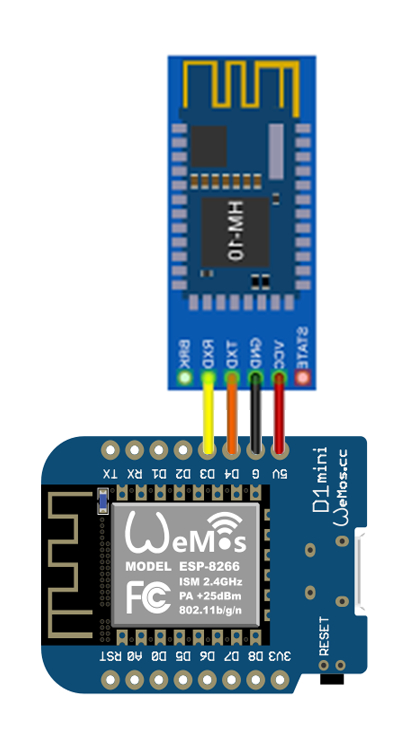
\includegraphics[width=0.3\linewidth]{central}
    \caption{Ligação dos componentes da central.}
    \label{fig:central}
\end{figure}

O \textit{software} que roda na central, baseado na Figura \ref{fig:blocos}, é detalhado no Listing \ref{list:main} abaixo.

\begin{lstlisting}[label={list:main},caption=Código-Fonte rodando no ESP8266.]
#include <SoftwareSerial.h>
#include <ESP8266WiFi.h>
#include <ESP8266WebServer.h>
#include <EEPROM.h>
#include <MQTTClient.h>

//EEPROM
#define PASSWORD_LENGTH_MAX 99
#define PASSWORD_ADDRESS_INIT 100   //101~199
#define SSID_LENGTH_MAX 99
#define SSID_ADDRESS_INIT 200       //201~299

#define BUFFER_LENGTH 600

//                 TX, RX
SoftwareSerial ble(D4, D3);       // For Uno, HM10 TX pin to Arduino Uno pin D2, HM10 RX pin to Arduino Uno pin D3
//SoftwareSerial ble(10,11);      // For Mega 2560, HM10 TX pin to Arduino Mega 2650 pin D10, HM10 RX pin to Arduino Mega 2560 pin D11

char buffer[BUFFER_LENGTH];       // Buffer to store response
char buffer2[BUFFER_LENGTH];       // Buffer to store response
int timeout = 800;          // Wait 800ms each time for BLE to response, depending on your application, adjust this value accordingly
long bauds[] = {115200, 9600, 57600, 38400, 2400, 4800, 19200}; // common baud rates, when using HM-10 module with SoftwareSerial, try not to go over 57600
long endTimeGetBeacon = 0;

long sum = 0;
long nums = 0;

ESP8266WebServer server(80);
WiFiClient wifi;

unsigned int id;

unsigned long wifi_time = 0;
unsigned long mqtt_time = 0;
unsigned long disp_time = 0;
unsigned long accp_time = 0;
unsigned long rfid_time = 0;
unsigned long  ble_time = 0;

byte wifi_status = 0;
byte mqtt_status = 0;
byte rfid_status = 0;
byte  ble_status = 0;

//TODO: Change to EEPROM
const char* clientId    = "porteiro";
const char* stremId     = "47677a26";
const char* privateKey  = "47677a26";
//TODO: Change to EEPROM
const char* brocker     = "52.67.131.199";
const char* mqttUser    = "mqttuser";
const char* mqttPass    = "mqttpassword";

MQTTClient mqtt; // manage MQTT conection with the server

long BLEAutoBaud() { // test each baudrate for finding the best for comunicating with HM10
  int baudcount = sizeof(bauds) / sizeof(long);
  for (int i = 0; i < baudcount; i++) {
    for (int x = 0; x < 3; x++) { // test at least 3 times for each baud
      Serial.print("Testing baud ");
      Serial.println(bauds[i]);
      ble.begin(bauds[i]);
      if (BLEIsReady()) {
        return bauds[i];
      }
    }
  }
  return -1;
}

boolean BLEIsReady() {
  BLECmd(timeout, "AT" , buffer);   // Send AT and store response to buffer
  if (strcmp(buffer, "OK") == 0) {
    return true;
  } else {
    return false;
  }
}

boolean BLECmd(long timeout, char* command, char* temp) {
  long endtime;
  boolean found = false;
  endtime = millis() + timeout; //
  memset(temp, 0, BUFFER_LENGTH);       // clear buffer
  found = true;
  Serial.print("Arduino send = ");
  Serial.println(command);
  ble.print(command);

  // The loop below wait till either a response is received or timeout
  // The problem with this BLE Shield is the HM-10 module does not response with CR LF at the end of the response,
  // so a timeout is required to detect end of response and also prevent the loop locking up.

  while (!ble.available()) {
    ESP.wdtFeed();
    if (millis() > endtime) {   // timeout, break
      found = false;
      break;
    }
  }

  if (found) {            // response is available
    int i = 0;
    while (ble.available()) {   // loop and read the data
      char a = ble.read();
      // Serial.print((char)a); // Uncomment this to see raw data from BLE
      temp[i] = a;        // save data to buffer
      i++;
      if (i >= BUFFER_LENGTH) break; // prevent buffer overflow, need to break
      delay(1);           // give it a 2ms delay before reading next character
    }
    Serial.print("BLE reply    = ");
    Serial.println(temp);
    return true;
  } else {
    Serial.println("BLE timeout!");
    return false;
  }
}

void getiBeacon(char* temp, char* empty_temp) {

  long endtime;
  boolean found = false;
  endtime = millis() + 800;
  memset(temp, 0, BUFFER_LENGTH);       // clear buffer
  found = true;


  //OK+DISIS
  //OK+DISC:4C000215:10F86430134611E491910800200C9A66:00010001CA:73ACE1A533A2:-056
  //OK+DISCE

  //OK+DISC
  //4C000215
  //10F86430134611E491910800200C9A66
  //00020001C8
  //5821A36D8BF1
  //-074

         // clear buffer
  Serial.println("S");
  delayMicroseconds(80);
  transmiteReceiveMessage("AT+DISI?", 1500, temp); 
  if (strcmp (temp, "OK+DISIS") == 0) {
  } else {
    Serial.println("E1!");
    return;
  }
  while (1) {
    if (!receiveMessage(4000, temp)) {
      Serial.println("E2!");
      break;
    } else {
      if (strcmp (temp, "OK+DISCE") == 0) {
        Serial.println("Terminou!");
        break;
      } else {
        Serial.println("Enviado");
      }
    }
    ESP.wdtFeed();
  }
}

bool transmiteReceiveMessage(char* command, long timeout, char* temp) {
  long endtime;
  boolean found = false;
  endtime = millis() + timeout; //
  memset(temp, 0, BUFFER_LENGTH);       // clear buffer
  found = true;
  ble.print(command);

  while (!ble.available()) {
    ESP.wdtFeed();
    if (millis() > endtime) {   // timeout, break
      found = false;
      break;
    }
  }

  if (found) {            // response is available
    int i = 0;
    while (ble.available()) {   // loop and read the data
      char a = ble.read();
      // Serial.print((char)a); // Uncomment this to see raw data from BLE
      temp[i] = a;        // save data to buffer
      i++;
      if (i >= BUFFER_LENGTH) break; // prevent buffer overflow, need to break
      delayMicroseconds(80);           // give it a 2ms delay before reading next character
    }
    return true;
  } else {
    Serial.println("BLE timeout!");
    return false;
  }
}

bool receiveMessage(long timeout, char* temp) {
  long endtime = millis() + timeout;
  boolean found = true;
  memset(temp, 0, BUFFER_LENGTH);
  
  while (!ble.available()) {
    ESP.wdtFeed();
    if (millis() > endtime) {   // timeout, break
      found = false;
      break;
    }
  }

  if (found) {
    int i = 0;
    while (ble.available()) {   // loop and read the data
      char a = ble.read();
      temp[i] = a;        // save data to buffer
      i++;
      if (i >= BUFFER_LENGTH) break; // prevent buffer overflow, need to break
      delayMicroseconds(80);           // give it a 2ms delay before reading next character
    }

    return true;

  } else {
    Serial.println("BLE timeout!");
    return false;
  }
}

void setup() {

  Serial.begin(115200);

  ESP.wdtEnable(15000);

  pinMode(13, OUTPUT);
  digitalWrite(13, LOW);

  Serial.println("Configuring WiFi...");
  connectWiFi();

  Serial.println("Configuring MQTT...");
  setupMQTT();


  BLECmd(timeout, "AT+NAME?", buffer);
  BLECmd(timeout, "AT+BAUD?", buffer);
  BLECmd(timeout, "AT+MODE?", buffer);
  BLECmd(timeout, "AT+PASS?", buffer);
  BLECmd(timeout, "AT+VERS?", buffer);
  BLECmd(timeout, "AT+RADD?", buffer);
  BLECmd(timeout, "AT+ADDR?", buffer);
  BLECmd(timeout, "AT+TYPE?", buffer);
  BLECmd(timeout, "AT+POWE?", buffer);
  BLECmd(timeout, "AT+NOTI1", buffer);
  Serial.println("----------------------");
  Serial.println("Configure...");
  BLECmd(timeout, "AT+ROLE1", buffer);
  BLECmd(timeout, "AT+IMME1", buffer);
  BLECmd(timeout, "AT+RESET ", buffer);
  Serial.println("----------------------");
  Serial.println("Waiting for remote connection...");


  endTimeGetBeacon = millis() + 3000;
}

void loop() {
  ESP.wdtFeed();
  loopWiFi();
  loopMQTT();
  if (WiFi.status() == WL_CONNECTED && wifi_status == 3) {
    if (mqtt.connected() && mqtt_status == 2) {
      loopBLE();
    }
  }
}


void loopBLE(){
  if (ble_status == 0) {
    Serial.println("BLE: Finding Baud Rate...");
    long baudrate = BLEAutoBaud();
    if (baudrate > 0) {
      Serial.print("BLE: Found baud rate ");
      Serial.println(baudrate);
      ble_status = 1; //found
    } else {
      Serial.println("BLE: No detected.");
      ble_time = millis();
    }
  } else if (wifi_status == 1) {
    if (millis() - wifi_time < 10000) {
      if (WiFi.status() != WL_CONNECTED) {
        if (millis() - disp_time > 500) {
          Serial.print(".");
          disp_time = millis();
        }
        if (millis() - accp_time > 120000) {
          Serial.println("\nWifi: Change to Access Point.");
          accp_time = millis();
          wifi_status = 5;
        }
      } else {
        wifi_status = 3; //connected
        Serial.print("\nWiFi: Connected. IP: ");
        Serial.println(WiFi.localIP());
        //        setupMQTT();
      }
    } else {
      Serial.println("\nWifi: Time out! Waiting for the next connection.");
      wifi_status = 4; //wait next connection
    }
  } else if (wifi_status == 3) {
    if (WiFi.status() != WL_CONNECTED) {
      Serial.println("Wifi: Connection lost.");
      wifi_status = 0;
    }
  } else if (wifi_status == 4) {
    if (millis() - wifi_time > 20000) {
      wifi_status = 1; //not connected
    }
  } else if (wifi_status == 5) {
    WiFi.softAP("Sensor");
    IPAddress apip = WiFi.softAPIP();
    server.on("/post", HTTP_POST, post);
    server.begin();
    Serial.print("Wifi: HTTP server beginned. IP: ");
    Serial.println(apip);
    wifi_status = 6;
  } else if (wifi_status == 6) {
    server.handleClient();
    if (millis() - accp_time > 120000) {
      Serial.println("Wifi: Change to Station WiFi.");
      accp_time = millis();
      wifi_status = 7;
    }
  } else if (wifi_status == 7) {
    connectWiFi();
  }

  
  if (ble.available()) {
    char c = (char)ble.read();
    Serial.print(c);
    if (c == '1') digitalWrite(LED_BUILTIN, HIGH); // if received character 1 from BLE, set PIN 13 high
    if (c == '0') digitalWrite(LED_BUILTIN, LOW); // if received character 0 from BLE, set PIN 13 low
  } else {
    if (millis() > endTimeGetBeacon) {
      endTimeGetBeacon = millis() + 1000;
      getiBeacon(buffer, buffer2);
    }
  }
}




void post() {
  String ssid1 = server.arg("ssid");
  String password1 = server.arg("password");
  if (id == server.arg("id").toInt()) {
    Serial.println(ssid1);
    Serial.println(password1);
    EEPROM.begin(4096);
    EEPROM.write(SSID_ADDRESS_INIT, ssid1.length());
    for (int i = 0; i < SSID_LENGTH_MAX; i++) {
      if (i > ssid1.length()) {
        EEPROM.write(SSID_ADDRESS_INIT + i + 1, '\0');
      } else {
        EEPROM.write(SSID_ADDRESS_INIT + i + 1, ssid1[i]);
      }
    }

    EEPROM.write(PASSWORD_ADDRESS_INIT, password1.length());
    for (int i = 0; i < PASSWORD_LENGTH_MAX; i++) {
      if (i > password1.length()) {
        EEPROM.write(PASSWORD_ADDRESS_INIT + i + 1, '\0');
      } else {
        EEPROM.write(PASSWORD_ADDRESS_INIT + i + 1, password1[i]);
      }
    }
    EEPROM.end();
    wifi_status = 7;
    server.send(200, "text/html", "OK");
  } else {
    wifi_status = 7;
    server.send(200, "text/html", "ERROR");
  }
}

void handleRoot() {
  server.send(200, "text/html", "");
}



void loopWiFi() {
  if (wifi_status == 0) {
    accp_time = millis();
    wifi_status = 1; //not connected
  } else if (wifi_status == 1) {
    Serial.println("WiFi: Connecting...");
    WiFi.begin();
    wifi_status = 2; //connecting
    wifi_time = millis();
  } else if (wifi_status == 2) {
    if (millis() - wifi_time < 10000) {
      if (WiFi.status() != WL_CONNECTED) {
        if (millis() - disp_time > 500) {
          Serial.print(".");
          disp_time = millis();
        }
        if (millis() - accp_time > 120000) {
          Serial.println("\nWifi: Change to Access Point.");
          accp_time = millis();
          wifi_status = 5;
        }
      } else {
        wifi_status = 3; //connected
        Serial.print("\nWiFi: Connected. IP: ");
        Serial.println(WiFi.localIP());
        //        setupMQTT();
      }
    } else {
      Serial.println("\nWifi: Time out! Waiting for the next connection.");
      wifi_status = 4; //wait next connection
      wifi_time = millis();
    }
  } else if (wifi_status == 3) {
    if (WiFi.status() != WL_CONNECTED) {
      Serial.println("Wifi: Connection lost.");
      wifi_status = 0;
    }
  } else if (wifi_status == 4) {
    if (millis() - wifi_time > 20000) {
      wifi_status = 1; //not connected
    }
  } else if (wifi_status == 5) {
    WiFi.softAP("Sensor");
    IPAddress apip = WiFi.softAPIP();
    server.on("/post", HTTP_POST, post);
    server.begin();
    Serial.print("Wifi: HTTP server beginned. IP: ");
    Serial.println(apip);
    wifi_status = 6;
  } else if (wifi_status == 6) {
    server.handleClient();
    if (millis() - accp_time > 120000) {
      Serial.println("Wifi: Change to Station WiFi.");
      accp_time = millis();
      wifi_status = 7;
    }
  } else if (wifi_status == 7) {
    connectWiFi();
  }
}




void connectWiFi() {
  EEPROM.begin(4096);
  int ssid_length = EEPROM.read(SSID_ADDRESS_INIT);
  if (ssid_length > SSID_LENGTH_MAX) {
    ssid_length = 0;
  }
  char *ssid = (char *)malloc(ssid_length + 1);
  for (int i = 0; i < ssid_length; i++) {
    ssid[i] = EEPROM.read(SSID_ADDRESS_INIT + i + 1);
  }
  ssid[ssid_length] = '\0';

  int password_length = EEPROM.read(PASSWORD_ADDRESS_INIT);
  if (password_length > PASSWORD_LENGTH_MAX) {
    password_length = 0;
  }
  char *password = (char *)malloc(password_length + 1);
  for (int i = 0; i < password_length; i++) {
    password[i] = EEPROM.read(PASSWORD_ADDRESS_INIT + i + 1);
  }
  password[password_length] = '\0';
  EEPROM.end();

  Serial.printf("SSID: '%s'(%d)\n", ssid, ssid_length);
  Serial.printf("Password: '%s'(%d)\n", password, password_length);

  WiFi.mode(WIFI_STA);
  WiFi.begin(ssid, password);

  wifi_status = 0;
}

void loopMQTT() {
  if (WiFi.status() != WL_CONNECTED || wifi_status != 3) {
    if (mqtt_status != 0 && mqtt_status != 5) {
      mqtt.disconnect();
      Serial.println("MQTT: Disconnected.");
      mqtt_status = 0;
    }
    return;
  }

  if (mqtt_status == 0) {
    mqtt.connect(clientId, mqttUser, mqttPass);

    Serial.println("MQTT: Connecting...");
    mqtt_status = 1; //connecting
    mqtt_time = millis();
  } else if (mqtt_status == 1) {
    if (millis() - mqtt_time < 10000) {
      if (!mqtt.connected()) {
        if (millis() - disp_time > 500) {
          Serial.print(".");
          disp_time = millis();
        }
      } else {
        mqtt_status = 2; //connected
        Serial.println("\nMQTT: Connected.");
        Serial.println("\nMQTT: Subscribe.");
        mqtt.subscribe("/door/1");
        mqtt.subscribe("/light/1");
        mqtt.subscribe("/setting/card");
        mqtt.subscribe("/setting/reset");
      }
    } else {
      Serial.println("\nMQTT: Time out!");
      Serial.println("\tWaiting for the next connection.");
      mqtt_status = 3; //wait next connection
    }
  } else if (mqtt_status == 2) {
    if (!mqtt.connected()) {
      Serial.println("MQTT: Connection lost.");
      Serial.println("\tWaiting for the next connection.");
      mqtt_status = 3; //wait next connection
    } else {
      mqtt.loop();
    }
  } else if (mqtt_status == 3) {
    if (millis() - mqtt_time > 20000) {
      mqtt_status = 0; //not connected
    }
  }
}

void setupMQTT() {
  Serial.println("MQTT: setting up.");
  mqtt = MQTTClient();
  mqtt.begin(brocker, wifi);
  mqtt.publish("rfid_reader/resetReason", ESP.getResetReason());
  Serial.println("MQTT: Configured.");
}


void messageReceived(String topic, String payload, char *bytes, unsigned int length) {
  Serial.print("Topic: ");
  Serial.println(topic);
  Serial.print("Payload: ");
  Serial.println(payload);
}






// MARK: Helper Functions

//one hex digit in ascii to an int
int htoi (char c) {  //does not check that input is valid
   if (c<='9')
       return c-'0';
   if (c<='F')
       return c-'A'+10;
   if (c<='f')
       return c-'a'+10;
   return 0;
}

int strH2Int (int start, int finish,char* temp) { 
  int result = 0;
   for(int i = start; i < finish+1; i++){
      result += (ipow(16,(finish-i))*htoi(temp[i]));
   }
   return result;
}

int ipow(int base, int exp) {
    int result = 1;
    while (exp) {
        if (exp & 1)
            result *= base;
        exp >>= 1;
        base *= base;
    }
    return result;
}
\end{lstlisting}

No sistema, três centrais são responsáveis pela triangulação do \textit{iBeacon}, monitorando seu distanciamento. No cenário de uma empresa, o ideal é colocá-las numa posição de entrada e saída de pessoas, local de fluxo dos funcionários quando estiverem indo levar os dispositivos para fora ou estiverem voltando com eles.

\begin{figure}[t!]
    \centering
    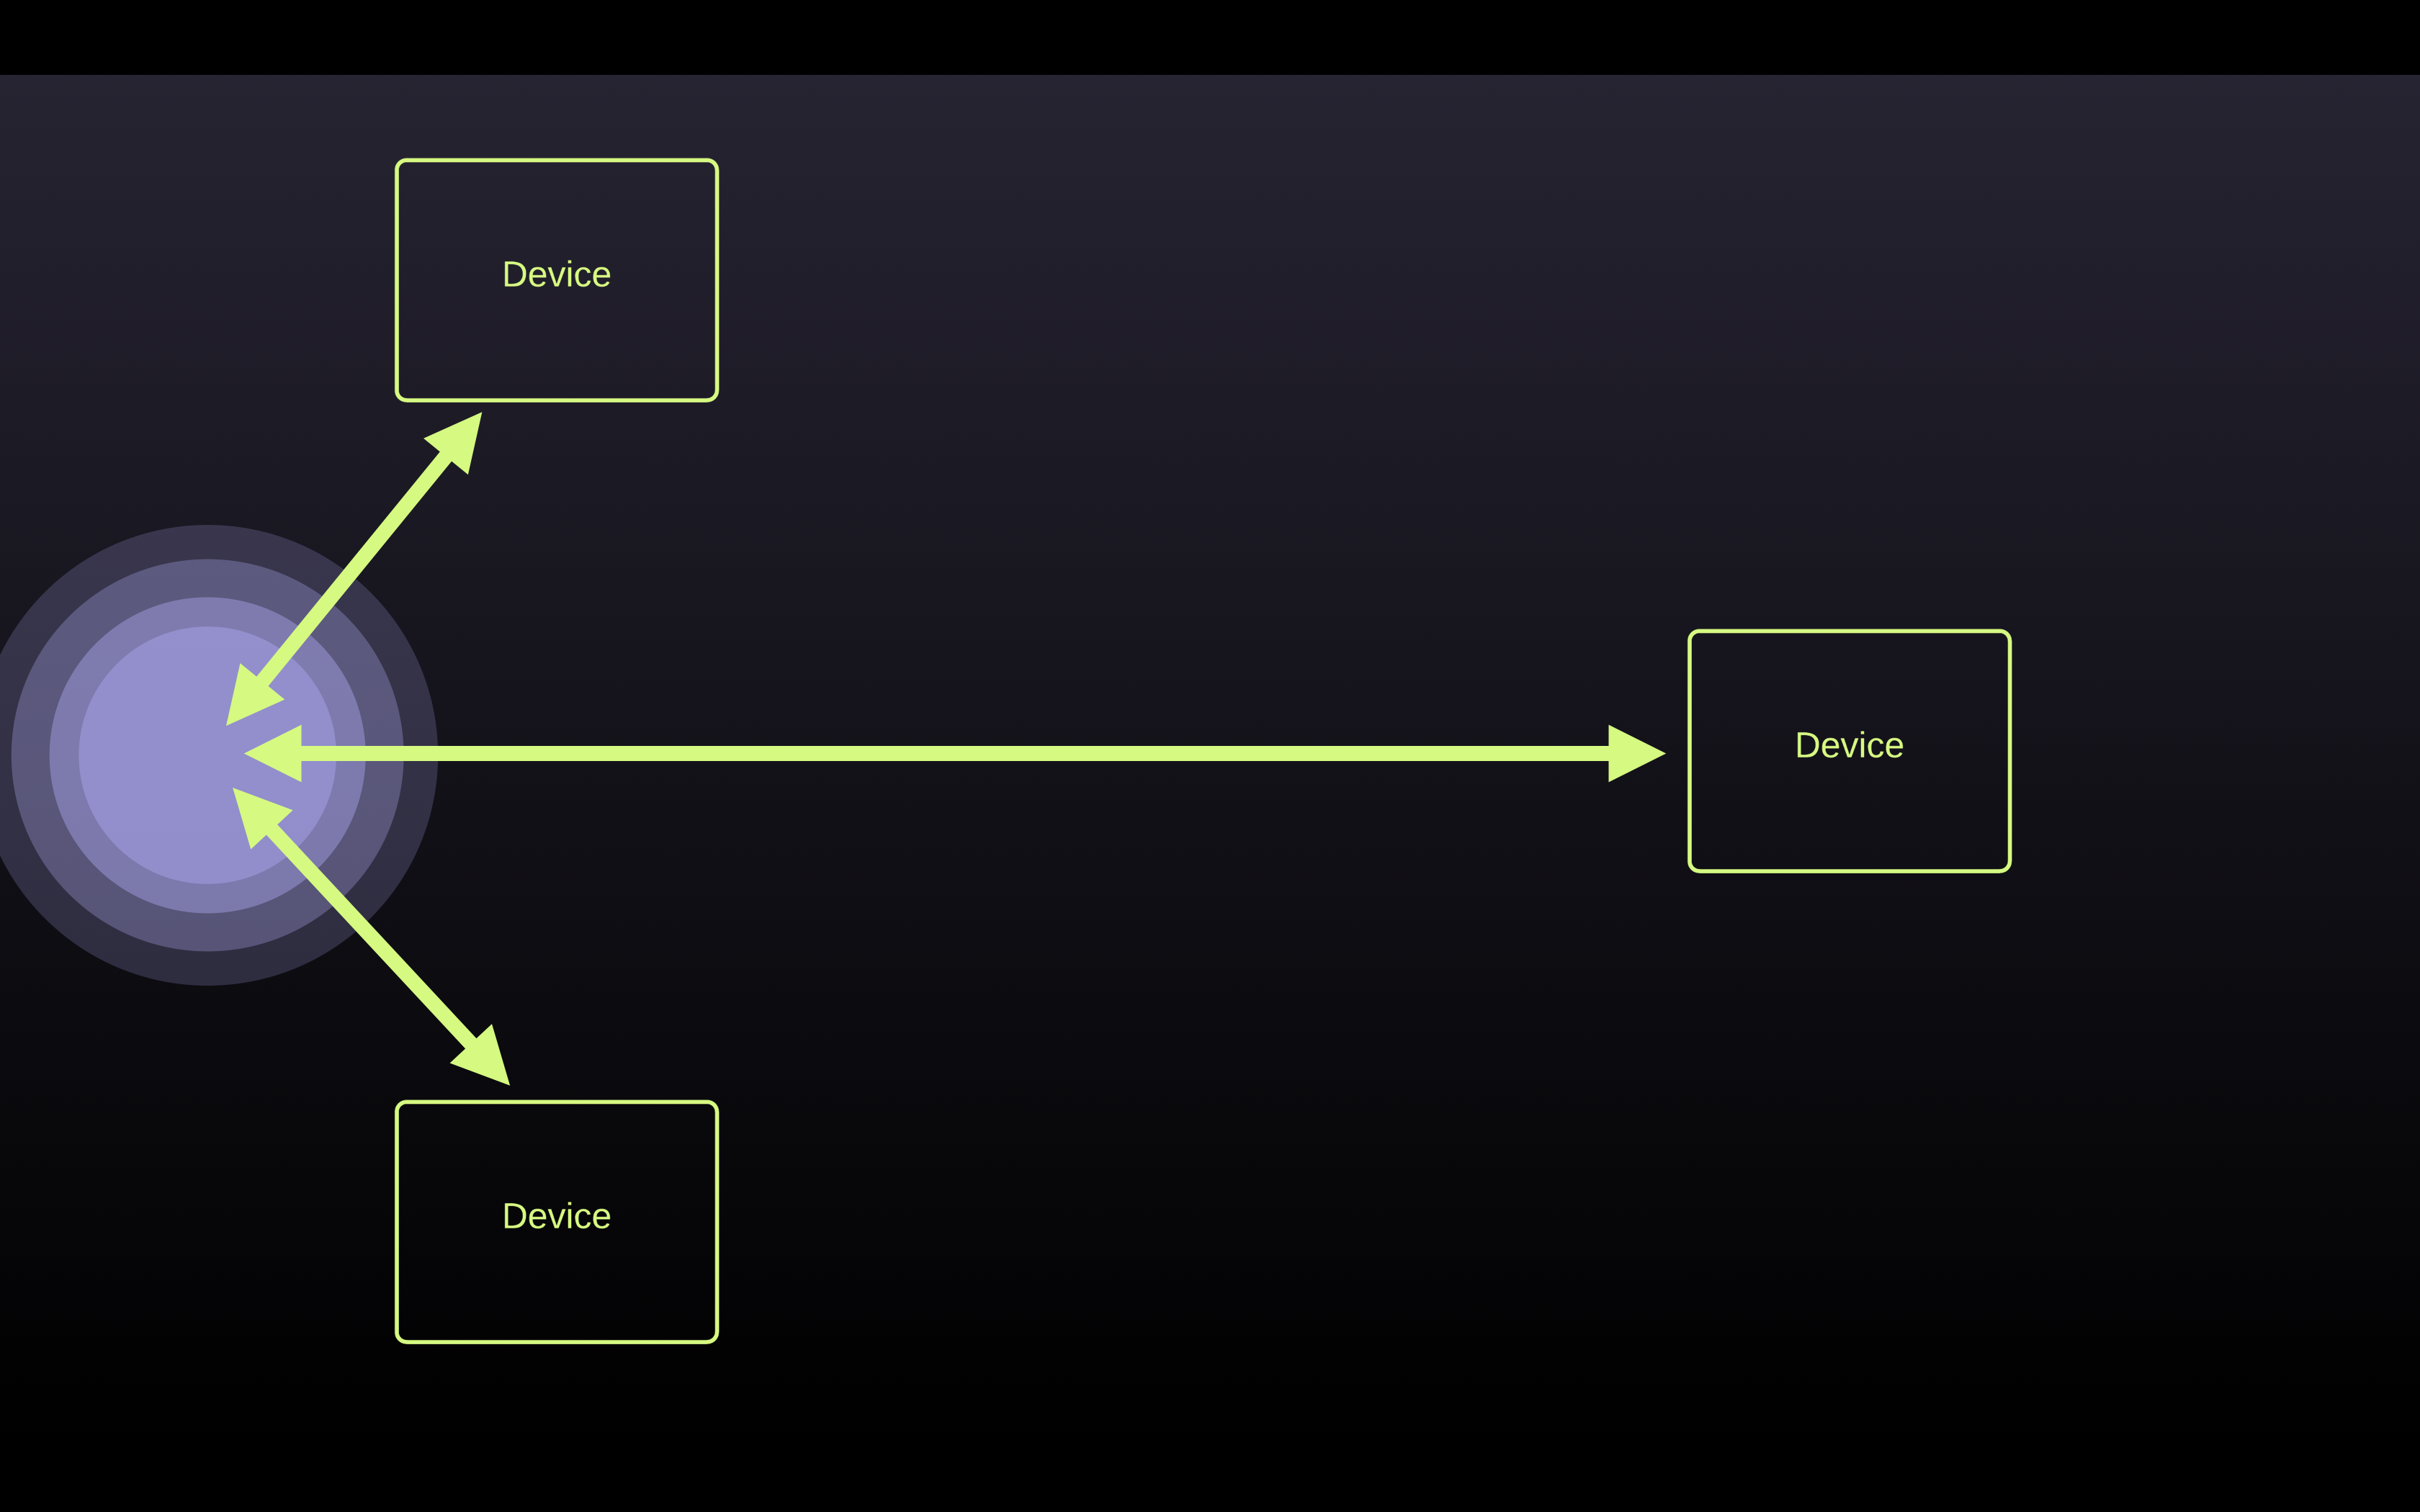
\includegraphics[width=0.7\linewidth]{system}
    \caption{Triangulação do \textit{iBeacon}.}
    \label{fig:system}
\end{figure}

\newpage

\section{Servidor}

O servidor, que comunica-se com as centrais pelo protocolo MQTT, já detalhado anteriormente e sem muitos segredos, seguindo o código fonte colocado no Listing \ref{list:server} abaixo. No exemplo didático elaborado no escopo atual, ele apenas mostra via \textit{console} o que foi recebido caso a mensagem seja compatível com o \textit{regex} colocado, seguindo assim um padrão.

\begin{lstlisting}[label={list:server},caption=Código-Fonte rodando no servidor.]
"use strict";
var mosca = require('mosca');
var settings = {
};

var data = {}

var server = new mosca.Server(settings);

var StringDecoder = require('string_decoder').StringDecoder;

server.on('clientConnected', function(client) {
    console.log('client connected', client.id);
});

// fired when a message is received
server.on('published', function(packet, client) {
    var decoder = new StringDecoder('utf8');
  console.log('Published', packet.topic, packet.payload);
  console.log(decoder.write(packet.payload));
const regex = /OK\+DISC\:(\w{3,8})\:(\w{3,60})\:(\w{3,60})\:(\w{3,60})\:-(\w{3,60})/g;
const str = decoder.write(packet.payload);
let m;

while ((m = regex.exec(str)) !== null) {
    // This is necessary to avoid infinite loops with zero-width matches
    if (m.index === regex.lastIndex) {
        regex.lastIndex++;
    }

    // The result can be accessed through the `m`-variable.
    m.forEach((match, groupIndex) => {
        if (groupIndex == 5) {
            data[packet.topic] = match
        }

        //console.log(`Found match, group ${groupIndex}: ${match}`);
    });
}
});

server.on('ready', setup);

// fired when the mqtt server is ready
function setup() {
  console.log('Mosca server is up and running');
}

module.exports = server;
\end{lstlisting}

\part{Discussão}

\chapter{Complicações}

Algumas complicações e atualizações foram necessárias durante o desenvolvimento do projeto, apresentando pequenos desafios que são parte do cotidiano da Engenharia. 

\section{\textit{Firmware} do HM10}

A versão do \textit{firmware} que veio com o módulo adquirido possuía menos funções, dificultando um pouco a localização de um \textit{iBeacon}. Sendo assim, foi necessário submeter o módulo a uma atualização (permitindo mais funções que permitiram localizar as \textit{tags}), que pode ser verificada nos repositórios do Github de \citeonline{firmware} e \citeonline{loader}. O primeiro contém o código fonte necessário e o segundo possui o código do Arduino necessário para gravação no módulo, segundo a Figura \ref{fig:firmware}.

\begin{figure}[h!]
    \centering
    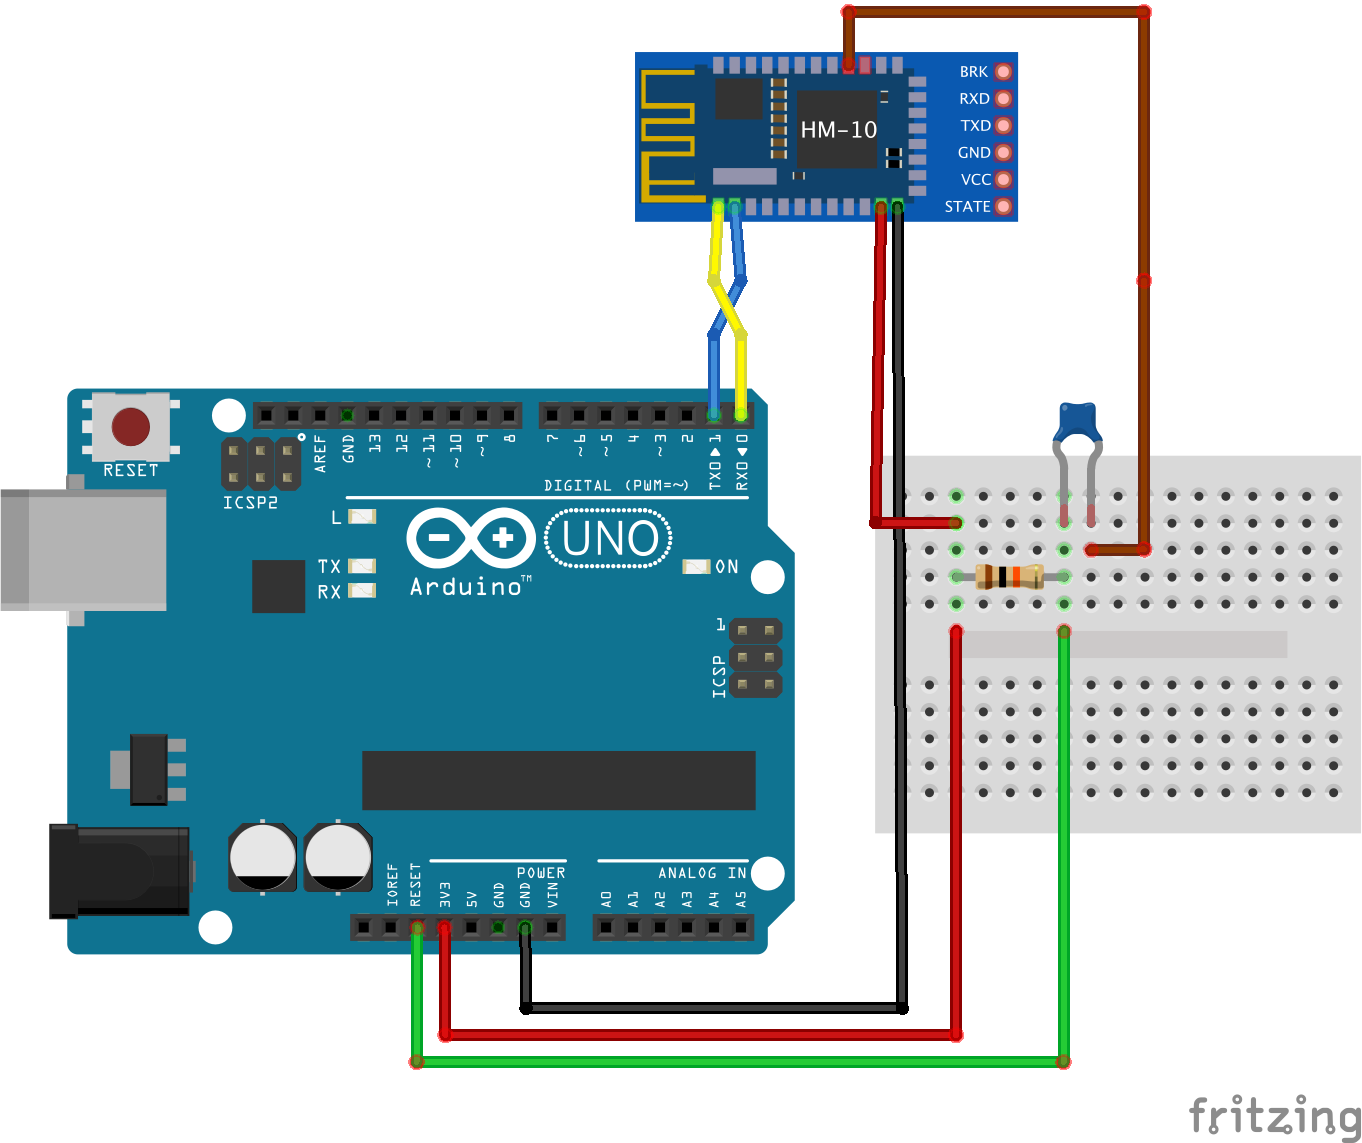
\includegraphics[width=0.6\linewidth]{firmware}
    \caption{Gravação do \textit{firmware} no HM10.}
    \label{fig:firmware}
\end{figure}

\section{Hospedagem no AWS}

Para conveniência durante a apresentação, dado que a conexão da universidade poderia dificultar a comunicação com o servidor, sem contar a autenticação, o servidor foi hospedado dentro de um \textit{Raspberry Pi} com todos os requisitos de instalação de uma máquina virtual (Linux OS, npm, git, etc). Um roteador simples da D-Link acompanha o conjunto para permitir a conexão ao respectivo IP.

\section{Atualização de dados do HM10}

Infelizmente, mesmo com a rapidez de comunicação e atualização do servidor, do protocolo MQTT e do ESP8266, o módulo HM10 apresentou lentidão em sua atualização de dados, apresentando erros de amostragem dos valores de distância do \textit{iBeacon}. Para uma captação ideal, seria necessária uma movimentação lenta da \textit{tag}, realizando um trajeto de um segundo em três minutos. 

Além disso, qualquer obstáculo colocado entre o BLE emissor e o módulo também causa erros de leitura. Todas estas complicações são provenientes da qualidade do \textit{hardware} adotado e podem ser solucionadas através de material mais avançado. 

Por exemplo, o \textit{hardware Bluetooth} de um \textit{iPhone} tem essa qualidade e, em testes entre o celular e um \textit{iBeacon}, a precisão se mantinha ainda que com velocidade e com obstáculos. Os mesmos resultados não puderam ser observados num celular rodando \textit{Android OS}, que apresentou os mesmos problemas citados, pois possuía equipamento inferior, talvez devido ao seu baixo custo.

\chapter{Conclusão}

O código-fonte, presente relatório e demais materiais podem ser acessados através do \textit{link} \url{https://drive.google.com/open?id=0B8ArAACUA-hORUM4ZTdMSGg2UlE}, estando um vídeo do \textit{YouTube} no \textit{link} \url{} demonstrando o funcionamento completo do sistema.

Após o desenvolvimento do sistema, um potencial negócio e futuras pesquisas podem ser desenvolvidas, explorando ainda mais a tecnologia de \textit{tags Bluetooth} que vem crescendo no mercado mundial com soluções de localização e controle, como pode ser observado nos artigos do IEEE Xplore de \citeonline{location} e de \citeonline{chair} e nas aplicações das empresas Tile, Tagpoint ou Estimote. Uma das principais aplicações para as quais o \textit{iBeacon} foi desenvolvido foi a localização precisa complementar ao GPS, além do lançamento de anúncios comerciais em lojas.

% ----------------------------------------------------------
% ELEMENTOS PÓS-TEXTUAIS
% ----------------------------------------------------------
\postextual
% ----------------------------------------------------------

% ----------------------------------------------------------
% Referências bibliográficas
% ----------------------------------------------------------
\bibliography{references}

%---------------------------------------------------------------------
% INDICE REMISSIVO
%---------------------------------------------------------------------
\phantompart
\printindex
%---------------------------------------------------------------------

\end{document}
